\chapter{Desarrollo embrionario de los vertebrados}\label{ch:b2:vertebrate-development}

Un huevo de rana es una esfera de dos milímetros de diámetro, oscura por
arriba y pálida por abajo. En un día se ha dividido en miles de células;
en dos, una lámina de esas células se ha enrollado hacia dentro a través
de un surco para formar un intestino y tender una varilla a lo largo del
dorso; en tres, la lámina situada sobre la varilla se ha plegado en un
tubo que será el encéfalo y la médula espinal. No se ha añadido nada más
que agua. La información que convierte una célula en un renacuajo
nadador estaba en el huevo y en su genoma, y la manera en que se despliega
--- \omterm{def:b2:vertebrate-development:egg}{segmentación}, gastrulación, neurulación, la \omterm{def:b2:vertebrate-development:induction}{inducción} de cada parte
por sus vecinas --- es reconociblemente la misma en un pez, un pollo y un
ratón. Este capítulo sigue a un embrión de vertebrado a través de esas
etapas y describe los experimentos que mostraron cómo se le indica a cada
una de sus partes lo que debe llegar a ser.

\section{Del huevo a la blástula}

\begin{definition}[El huevo y sus ejes]\label{def:b2:vertebrate-development:egg}
\index{polo animal}\index{polo vegetativo}\index{vitelo}\index{segmentación}
El huevo de un vertebrado está polarizado antes de la fecundación: el
\emph{polo animal} contiene el núcleo y la mayor parte del citoplasma; el
\emph{polo vegetativo}, el \emph{vitelo}, la reserva de proteínas y
lípidos de la que vivirá el embrión hasta que se alimente. La cantidad de
vitelo fija el patrón de todo lo que sigue: un huevo de erizo de mar o de
mamífero casi no tiene y se segmenta por completo en células iguales; un
huevo de rana tiene una cantidad moderada y se segmenta por completo pero
de forma desigual (células pequeñas arriba, grandes células cargadas de
vitelo abajo); un huevo de pez o de ave es casi todo vitelo y solo se
segmenta en un disco de citoplasma situado encima. En la rana, el punto
por el que entra el espermatozoide fija el segundo eje: la corteza gira
treinta grados alejándose de él y deja al descubierto una \emph{media
luna gris} opuesta al punto de entrada, y ese lado se convertirá en el
dorso. La \emph{segmentación} es una serie de mitosis rápidas sin
crecimiento --- las células se reducen a la mitad de tamaño en cada una
---, impulsada por ARNm y proteínas maternos almacenados en el huevo,
mientras los propios genes del embrión permanecen en silencio hasta la
\emph{transición de la \omterm{def:b2:vertebrate-development:blastula}{blástula} media}, al cabo de unas doce divisiones.
\end{definition}

\begin{omfigure}
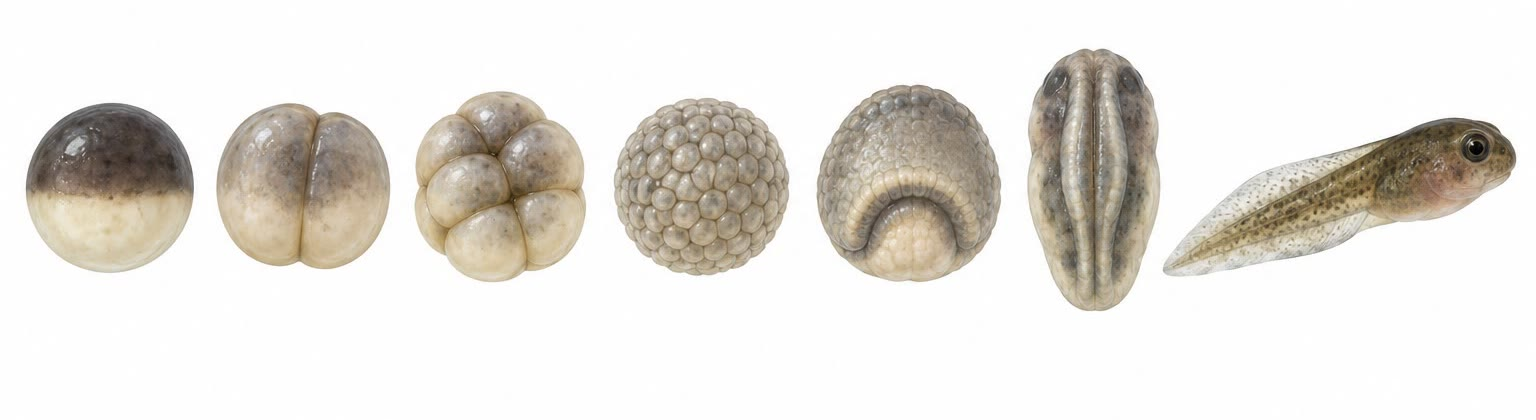
\includegraphics[width=0.9\linewidth]{images/book4/ai/b4-10-frog-development.jpg}

{\small El desarrollo de una rana desde el huevo fecundado: la
\omterm{def:b2:vertebrate-development:egg}{segmentación} hasta la \omterm{def:b2:vertebrate-development:blastula}{blástula}, la gastrulación, la néurula con sus
pliegues neurales y el renacuajo --- todo en unos pocos días, sin
crecimiento.}
\end{omfigure}

\begin{theorem}[La aritmética de la segmentación]\label{thm:b2:vertebrate-development:cleavage}
Tras $k$ \omterm{def:b2:vertebrate-development:egg}{segmentaciones} sincrónicas, un huevo de volumen $V_0$ son $2^{k}$
células de volumen medio $V_0/2^{k}$ y radio $r_0/2^{k/3}$, y la
superficie total ha crecido en un factor $2^{k/3}$; la relación entre el
volumen nuclear y el citoplasmático, que parte de cerca de $10^{-4}$ en un
huevo de rana, aumenta en un factor $2^{k}$ y alcanza la de una célula
ordinaria ($\sim 0.1$) al cabo de unas diez divisiones. Es esta relación
creciente --- la titulación de una reserva materna fija de algún
inhibidor por una cantidad de ADN que crece exponencialmente --- la que
desencadena la transición de la \omterm{def:b2:vertebrate-development:blastula}{blástula} media: las divisiones se
ralentizan, se vuelven asincrónicas y el genoma cigótico se activa.
\end{theorem}
\begin{proof}
El volumen se conserva en la \omterm{def:b2:vertebrate-development:egg}{segmentación}, de modo que cada una de las
$2^{k}$ células tiene $V_0
2^{-k}$ y, como esfera, un radio $r_0 2^{-k/3}$; su superficie total es
$2^{k}\cdot 4\pi r_0^{2}\, 2^{-2k/3} = 4\pi r_0^{2}\, 2^{k/3}$. Cada
célula conserva un núcleo de tamaño fijo, de modo que la relación crece
como $2^{k}$ desde $10^{-4}$: $2^{10} = 1024$ la lleva a $0.1$. La
transición de la rana se sitúa en la duodécima división, lo que es
coherente con un umbral alcanzado algo más tarde.
\end{proof}
\begin{proof}[Evidencia]
Newport y Kirschner (1982) añadieron ADN adicional a huevos de rana y
observaron que la transición se adelantaba tantas divisiones como veces
había ADN en exceso; eliminar citoplasma tenía el mismo efecto. El reloj
no es el tiempo ni un recuento de divisiones, sino una relación.
\end{proof}

\begin{definition}[Blástula]\label{def:b2:vertebrate-development:blastula}
\index{blástula}\index{blastocele}
La \omterm{def:b2:vertebrate-development:egg}{segmentación} termina en una \emph{blástula}: una esfera hueca (rana,
erizo de mar) o un disco (pez, ave) de unos pocos miles de células
alrededor de una cavidad, el \emph{blastocele}. Sus células tienen todavía
un aspecto no especializado, pero no son equivalentes: un \emph{mapa de
destinos}, construido tiñendo zonas de la superficie con colorantes y
siguiéndolas, muestra que el casquete animal dará la piel y el sistema
nervioso (\emph{ectodermo}), el cinturón ecuatorial el músculo, el
esqueleto, el riñón y la sangre (\emph{mesodermo}), y la masa vegetativa
el intestino y sus órganos (\emph{endodermo}). Estas tres \emph{hojas
embrionarias} son las mismas en todos los vertebrados, y el paso
siguiente es colocarlas en su sitio: el mesodermo y el endodermo están
fuera y deben entrar.
\end{definition}

\section{Gastrulación y neurulación}

\begin{proposition}[La gastrulación]\label{prop:b2:vertebrate-development:gastrulation}
\index{gastrulación}\index{blastoporo}\index{arquénteron}\index{notocorda}
La \emph{gastrulación} es el conjunto de movimientos celulares que
convierte la \omterm{def:b2:vertebrate-development:blastula}{blástula} de una sola capa en una \emph{gástrula} de tres
capas. En la rana empieza por debajo de la media luna gris: las células
cambian de forma y contraen su extremo externo en forma de botella, y la
superficie se hunde en un surco, el \emph{blastoporo}. A través de él el
mesodermo y el endodermo fluyen hacia dentro (\emph{involución}),
enrollándose sobre el labio y avanzando a lo largo del techo de la
cavidad; el casquete animal se extiende hacia abajo para cubrir el
exterior (\emph{epibolia}); el blastoporo se cierra en un anillo alrededor
de las últimas células vitelinas. Dentro, una nueva cavidad revestida de
endodermo, el \emph{arquénteron}, es el futuro intestino, y el mesodermo
que entró primero, a lo largo de la línea media, se ha convertido en una
varilla rígida, la \emph{notocorda}, el eje de todo embrión de vertebrado
y la estructura que da nombre al filo. En las aves y los mamíferos los
mismos movimientos se producen a través de una hendidura, la
\emph{línea primitiva}, en un disco plano; en los peces, el disco se
extiende sobre el \omterm{def:b2:vertebrate-development:egg}{vitelo}. La coreografía cambia con el \omterm{def:b2:vertebrate-development:egg}{vitelo}; el
resultado --- ectodermo fuera, endodermo revistiendo el intestino,
mesodermo entre ambos, notocorda en la línea media --- es el mismo.
\end{proposition}

\begin{omfigure}
\begin{tikzpicture}[every node/.style={font=\scriptsize}, >=stealth]
  % blastula
  \begin{scope}
    \draw[thick, fill=omDef!15] (0,0) circle (1.3);
    \draw[thick, fill=white] (0,0.2) circle (0.75);
    \fill[omExo!40] (0,0) ++(-1.3,0) arc (180:360:1.3 and 1.3) -- cycle;
    \draw[thick] (0,0) circle (1.3);
    \node at (0,0.2) {blastocele};
    \node[below, align=center] at (0,-1.45) {blástula\\casquete animal (azul), células vitelinas (gris)};
  \end{scope}
  % early gastrula: blastopore forming
  \begin{scope}[xshift=4.2cm]
    \draw[thick, fill=omDef!15] (0,0) circle (1.3);
    \draw[thick, fill=white] (0,0.25) circle (0.7);
    \fill[omExo!40] (0,0) ++(-1.3,0) arc (180:360:1.3 and 1.3) -- cycle;
    \draw[thick] (0,0) circle (1.3);
    \draw[very thick, omThm] (1.0,-0.85) .. controls (0.5,-0.6) and (0.4,-0.3) .. (0.55,0.0);
    \draw[->, thick, omThm] (1.15,-0.7) .. controls (0.6,-0.4) .. (0.4,0.1);
    \draw[omThm] (1.0,-0.85) -- (0.9,-1.25); \node[omThm, anchor=north west] at (0.6,-1.2) {labio del blastoporo};
    \node[below, align=center] at (0,-1.45) {gástrula temprana\\las células entran por el labio};
  \end{scope}
  % late gastrula
  \begin{scope}[xshift=8.4cm]
    \draw[thick, fill=omDef!15] (0,0) circle (1.3);
    \draw[thick, fill=omExo!25] (0,0.05) circle (0.95);
    \draw[thick, fill=white] (0.15,-0.1) ellipse (0.55 and 0.4);
    \draw (0.6,-0.3) -- (1.6,-1.15); \node[anchor=west] at (1.6,-1.15) {arquénteron};
    \draw[very thick, omThm] (-0.9,0.35) .. controls (-0.2,0.6) .. (0.8,0.4);
    \draw[omThm] (0.0,0.48) -- (-0.9,1.55); \node[omThm, anchor=east] at (-0.9,1.55) {notocorda};
    \draw[thick] (1.1,-0.7) -- (1.3,-0.5);
    \node[right] at (1.3,-0.5) {blastoporo};
    \node[below, align=center] at (0,-1.45) {gástrula tardía: tres capas,\\cavidad intestinal, notocorda en el techo};
  \end{scope}
\end{tikzpicture}

{\small La gastrulación en la rana, en sección. Las células se enrollan
hacia dentro sobre el labio del blastoporo; el endodermo reviste una nueva
cavidad intestinal, y el primer mesodermo en entrar se convierte en la
notocorda a lo largo de la línea media.}
\end{omfigure}

\begin{proposition}[La neurulación y el plan corporal]\label{prop:b2:vertebrate-development:neurulation}
\index{neurulación}\index{tubo neural}\index{somito}\index{cresta neural}
El ectodermo situado sobre la notocorda se engrosa en una \emph{placa
neural}, cuyos bordes se elevan en pliegues y se unen en la línea media
para formar el \emph{\omterm{prop:b2:vertebrate-development:neurulation}{tubo neural}}, el futuro encéfalo y médula espinal,
que se hunde bajo la piel; células de la cresta de los pliegues, la
\emph{\omterm{prop:b2:vertebrate-development:neurulation}{cresta neural}}, migran lejos para formar los nervios periféricos,
las células pigmentarias, la médula suprarrenal y gran parte de la cara.
A cada lado de la notocorda el mesodermo se segmenta en bloques, los
\emph{somitos}, un par tras otro de la cabeza a la cola, que dan las
vértebras, los músculos del tronco y la dermis; el mesodermo lateral se
divide en las capas que revisten la cavidad corporal y forman el corazón
y las extremidades; el tubo endodérmico forma por gemación los pulmones,
el hígado y el páncreas. Al final de la neurulación el embrión tiene el
plan corporal de los vertebrados --- un cordón nervioso dorsal sobre una
notocorda, un intestino ventral, músculo segmentado, una cabeza --- con
una longitud de unos pocos milímetros, y el resto del desarrollo es la
elaboración de los órganos a partir de ese plan
(\cref{ch:b2:limb-organogenesis}).
\end{proposition}

\begin{omfigure}
\begin{tikzpicture}[every node/.style={font=\scriptsize}]
  \foreach \x/\lab in {0/{placa neural}, 4.0/{se elevan los pliegues neurales}, 8.0/{tubo neural cerrado; migra la cresta neural}} {
    \begin{scope}[xshift=\x cm]
      \draw[thick, fill=omExo!25] (-1.6,0) rectangle (1.6,-1.6);
      \draw[thick, omThm, fill=omThm!30] (0,-0.75) circle (0.28);
      \draw[thick, fill=omProp!30] (-1.3,-0.75) circle (0.32); \draw[thick, fill=omProp!30] (1.3,-0.75) circle (0.32);
      \node[below, align=center, text width=3.4cm] at (0,-1.7) {\lab};
    \end{scope}
  }
  \draw[very thick, omDef] (-1.6,0) -- (-0.7,0) .. controls (-0.3,0.15) and (0.3,0.15) .. (0.7,0) -- (1.6,0);
  \draw[very thick, omDef] (2.4,0) -- (3.3,0) .. controls (3.3,0.9) and (3.6,0.1) .. (4.0,0.0) .. controls (4.4,0.1) and (4.7,0.9) .. (4.7,0) -- (5.6,0);
  \draw[very thick, omDef] (6.4,0.05) -- (9.6,0.05);
  \draw[very thick, omDef, fill=omDef!20] (8.0,-0.3) circle (0.3);
  \foreach \p in {(7.35,-0.4),(8.65,-0.4)} \fill[omDef!70!black] \p circle (0.07);
  \node[omThm, anchor=west] at (9.8,-0.75) {notocorda};
  \node[omProp, anchor=west] at (9.8,-1.15) {somito};
  \node[omDef, anchor=west] at (9.8,-0.3) {tubo neural};
  \node[omDef!70!black, anchor=west] at (9.8,0.1) {células de la cresta neural};
\end{tikzpicture}

{\small La neurulación en sección transversal: el ectodermo situado sobre
la notocorda (rojo) se engrosa, se pliega y se cierra en el \omterm{prop:b2:vertebrate-development:neurulation}{tubo neural}
(azul), mientras el mesodermo junto a la notocorda se segmenta en somitos
(naranja) y las células de la \omterm{prop:b2:vertebrate-development:neurulation}{cresta neural} abandonan los pliegues que
se cierran.}
\end{omfigure}

\begin{omfigure}
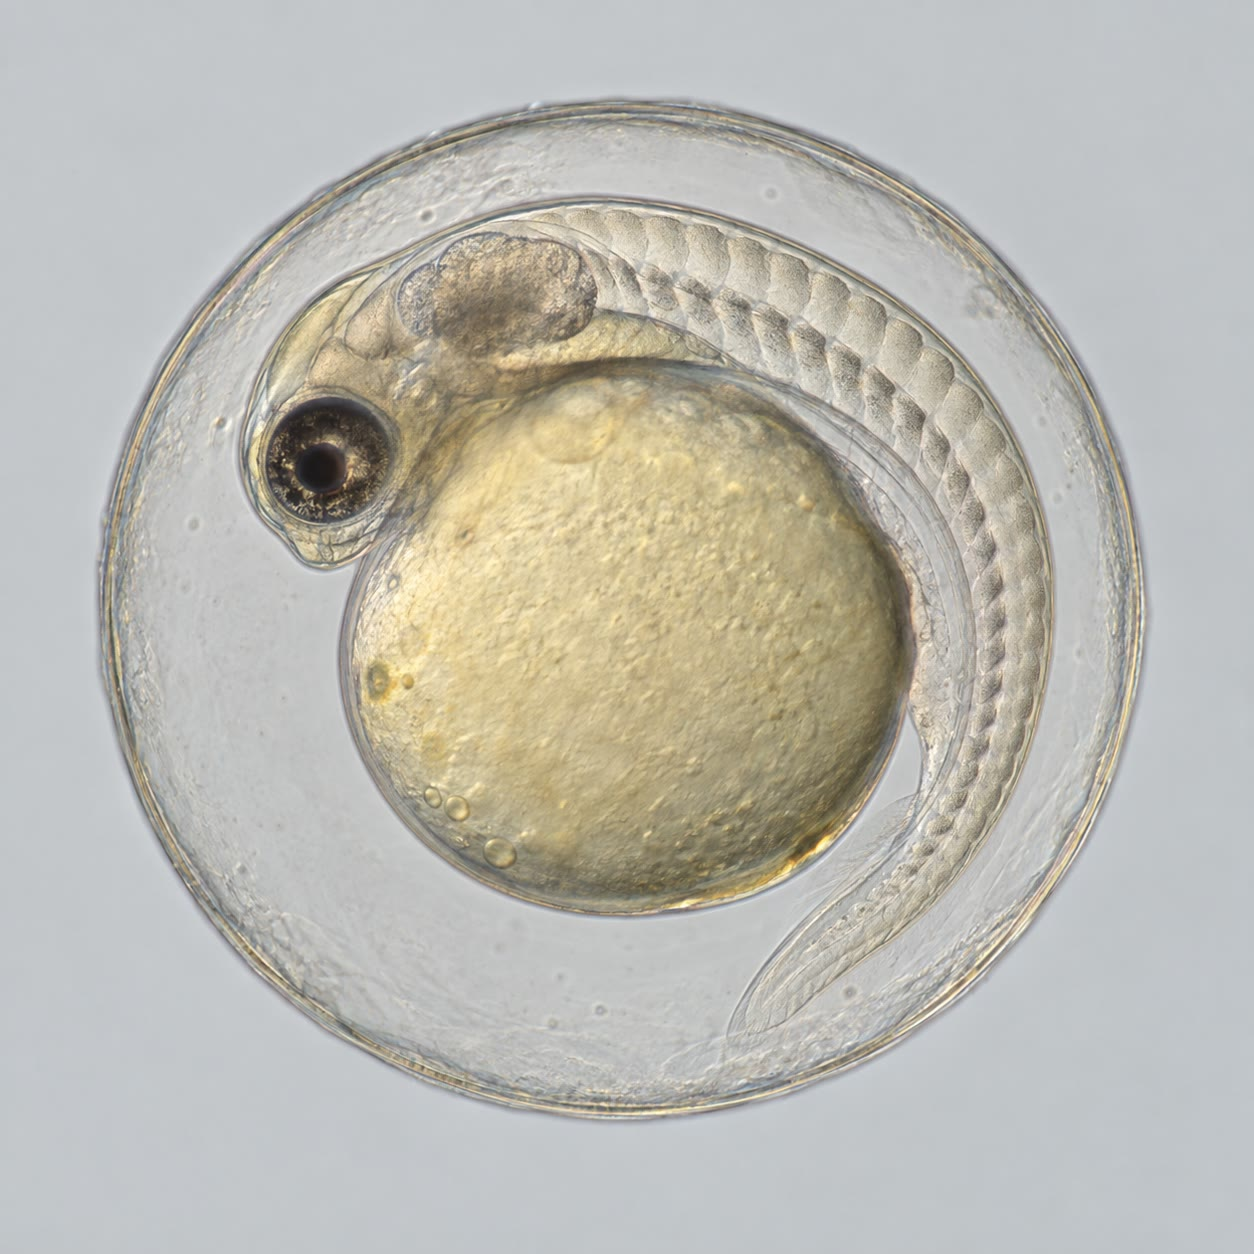
\includegraphics[width=0.42\linewidth]{images/book4/ai/b4-10-zebrafish-embryo.jpg}\hspace{0.04\linewidth}
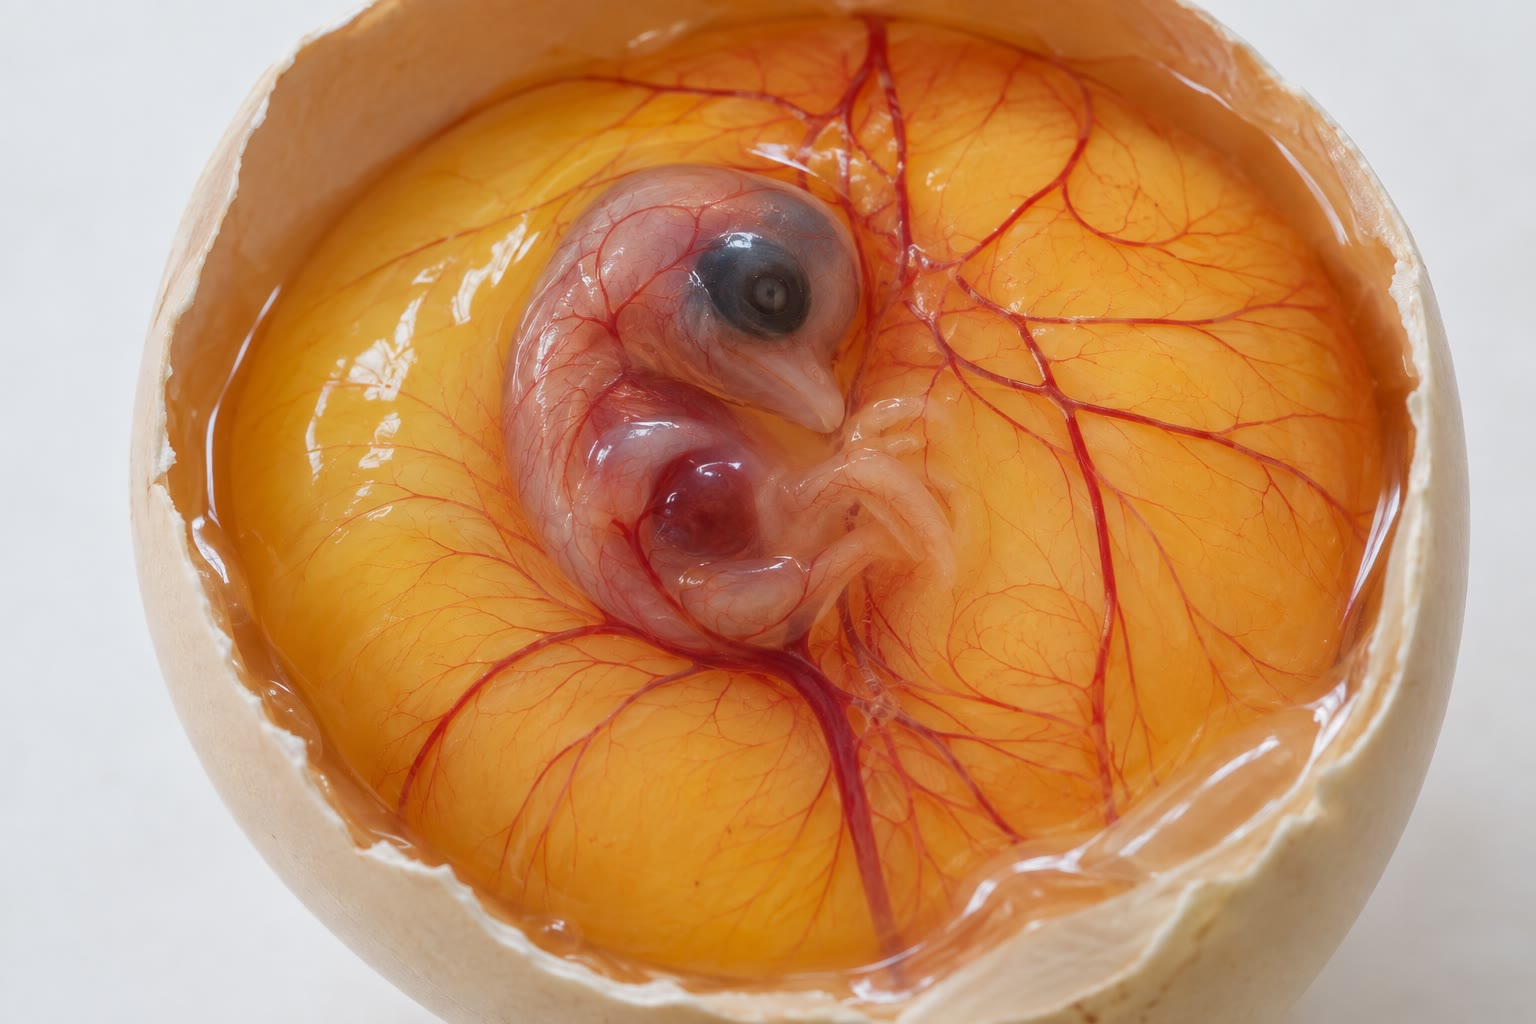
\includegraphics[width=0.5\linewidth]{images/book4/ai/b4-10-chick-embryo.jpg}

{\small Izquierda: un embrión de pez cebra de un día dentro de su corion,
enrollado alrededor de su \omterm{def:b2:vertebrate-development:egg}{vitelo}, con el ojo, el encéfalo y una hilera de
somitos. Derecha: un embrión de pollo de tres días sobre su \omterm{def:b2:vertebrate-development:egg}{vitelo}, con
el corazón ya latiendo y los vasos extendiéndose sobre el \omterm{def:b2:vertebrate-development:egg}{vitelo} para
alimentarlo.}
\end{omfigure}

\section{La inducción: cómo saben las células dónde están}

\begin{definition}[Inducción y competencia]\label{def:b2:vertebrate-development:induction}
\index{inducción (embrionaria)}\index{competencia}\index{organizador}
La \emph{inducción} es el proceso por el cual un grupo de células cambia
el destino de un grupo vecino mediante una señal; las células que
responden deben ser \emph{competentes} --- capaces de responder, lo que
solo son durante un tiempo limitado. El desarrollo es una cadena de
inducciones: las células vegetativas inducen mesodermo en las células
situadas sobre ellas; el mesodermo dorsal --- el \emph{organizador} del
labio del blastoporo --- induce la placa neural en el ectodermo situado
encima y organiza el mesodermo de ambos lados; la notocorda induce el
suelo del \omterm{prop:b2:vertebrate-development:neurulation}{tubo neural}; la vesícula óptica, una evaginación del encéfalo,
induce un cristalino en la piel que toca; el cristalino induce la córnea.
Cada tejido inducido se convierte en inductor del siguiente. Las señales
son un puñado de familias de proteínas secretadas que se usan una y otra
vez --- las mismas que organizan una extremidad
(\cref{ch:b2:limb-organogenesis}) y que, en el adulto, gobiernan la
señalización del \cref{ch:b2:cell-signalling}.
\end{definition}
\begin{proof}[Evidencia]
Spemann y Mangold (1924) cortaron el labio dorsal del blastoporo de una
gástrula temprana de una especie de tritón y lo injertaron en el lado
ventral de otra, de pigmentación diferente para poder distinguir las
células del huésped y las del injerto. El injerto no se limitó a
convertirse en lo que habría sido en su sitio: se enrolló hacia dentro,
formó notocorda e \emph{indujo al propio ectodermo ventral del huésped} a
formar un segundo \omterm{prop:b2:vertebrate-development:neurulation}{tubo neural} y, junto a él, somitos del huésped --- un
segundo embrión completo, formado en gran parte por células del huésped,
unido vientre con vientre al primero. Ningún otro fragmento de la
gástrula podía hacerlo. Llamaron al labio el \omterm{def:b2:vertebrate-development:induction}{organizador}; sus señales
(proteínas que bloquean el factor ventralizante BMP) se identificaron
setenta años después.
\end{proof}

\begin{omfigure}
\begin{tikzpicture}[every node/.style={font=\scriptsize}, >=stealth]
  % donor
  \draw[thick, fill=omDef!12] (0,0) circle (1.3); \node[above] at (0,1.4) {gástrula donante (pálida)};
  \draw[very thick, omThm] (0.85,-0.95) arc (-45:-20:1.3); \node[omThm, right] at (1.2,-0.8) {labio dorsal};
  \draw[->, thick] (1.6,-0.3) -- (3.4,-0.3);
  % host
  \draw[thick, fill=omExo!45] (5,0) circle (1.3); \node[above] at (5,1.4) {gástrula huésped (oscura)};
  \draw[very thick, omThm] (5.85,-0.95) arc (-45:-20:1.3); \node[omThm, right] at (6.2,-0.8) {labio propio};
  \draw[very thick, omThm] (4.15,0.95) arc (135:160:1.3); \node[omThm, left] at (3.9,1.0) {injerto};
  \draw[->, thick] (6.6,-0.3) -- (8.4,-0.3);
  % result: twinned embryo
  \draw[thick, fill=omExo!45] (10.6,0) ellipse (1.8 and 1.1);
  \draw[very thick, omDef!70!black] (9.2,0.5) .. controls (10.0,0.8) and (11.2,0.8) .. (12.0,0.5);
  \draw[very thick, omDef!70!black] (9.2,-0.5) .. controls (10.0,-0.8) and (11.2,-0.8) .. (12.0,-0.5);
  \node[above] at (10.6,1.2) {resultado: dos ejes};
  \node[anchor=north, align=center, text width=4cm] at (10.6,-1.2) {un segundo tubo neural y somitos, formados por células del \emph{huésped}, inducidos por el injerto};
\end{tikzpicture}

{\small El experimento del \omterm{def:b2:vertebrate-development:induction}{organizador}. Un labio dorsal injertado en el
vientre de otra gástrula induce a las células del huésped a formar un
segundo eje embrionario.}
\end{omfigure}

\begin{theorem}[Un gradiente de morfógeno]\label{thm:b2:vertebrate-development:gradient}
\index{morfógeno}
Muchas inducciones funcionan mediante un \emph{morfógeno}: una señal
secretada por una fuente, que se extiende por el tejido y que las células
leen según su concentración local --- por encima de un umbral, un
destino; por encima de otro más alto, otro distinto. Un morfógeno
producido en una fuente plana a un ritmo $j$ por unidad de superficie,
que difunde con coeficiente $D$ y se degrada a un ritmo $k$, tiene en
estado estacionario el perfil exponencial
\[
c(x) = c_0\,e^{-x/\lambda}, \qquad \lambda = \sqrt{D/k}, \qquad c_0 = \frac{j}{\sqrt{Dk}},
\]
de modo que la distancia a la que la concentración cae por debajo de un
umbral $T$ es $x_T = \lambda\ln(c_0/T)$: umbrales fijos pueden dividir un
tejido en bandas de anchura fija. Con $D =
\qty{1e-12}{m^2/s}$ (una proteína frenada por sus uniones al avanzar por
el tejido) y $k = \qty{1e-3}{s^{-1}}$ (una semivida de unos doce
minutos), $\lambda = \sqrt{10^{-9}}\,\unit{m} \approx
\qty{32}{\micro m}$: unos pocos diámetros celulares, la escala en la que
se organizan los campos embrionarios. Duplicar la fuente duplica $c_0$ y
desplaza cada frontera hacia fuera en $\lambda
\ln 2$.
\end{theorem}
\begin{proof}
En estado estacionario la difusión equilibra la degradación: $D\,c'' = k\,c$,
cuya solución decreciente es $c = c_0 e^{-x/\lambda}$ con $\lambda^2 =
D/k$. El flujo que sale de la fuente es $-Dc'(0) = Dc_0/\lambda = j$,
lo que da $c_0 = j\lambda/D = j/\sqrt{Dk}$. Imponiendo $c(x_T) = T$
se obtiene $x_T$; cambiar $c_0$ por $2c_0$ le suma $\lambda\ln 2$.
\end{proof}

\begin{omfigure}
\begin{tikzpicture}
\begin{axis}[
  width=0.78\linewidth, height=5.6cm,
  axis x line=bottom, axis y line=left,
  xmin=0, xmax=120, ymin=0, ymax=1.1,
  xlabel={distancia a la fuente (\unit{\micro m})}, ylabel={morfógeno (relativo)},
  xlabel style={font=\small, at={(axis description cs:0.5,-0.13)}, anchor=north},
  ylabel style={font=\small},
  tick label style={font=\small}, xtick={0,32,64,96}, ytick={0,0.5,1},
  clip=false,
]
\fill[omThm!18] (axis cs:0,0) rectangle (axis cs:22,1.05); \node[font=\scriptsize, anchor=south] at (axis cs:11,1.05) {destino A};
\fill[omProp!18] (axis cs:22,0) rectangle (axis cs:61,1.05); \node[font=\scriptsize, anchor=south] at (axis cs:41,1.05) {destino B};
\fill[omExo!18] (axis cs:61,0) rectangle (axis cs:120,1.05); \node[font=\scriptsize, anchor=south] at (axis cs:90,1.05) {destino C};
\addplot[very thick, omDef, domain=0:120, samples=80] {exp(-x/32)};
\draw[dashed, gray] (axis cs:0,0.5) -- (axis cs:22,0.5) -- (axis cs:22,0);
\draw[dashed, gray] (axis cs:0,0.15) -- (axis cs:61,0.15) -- (axis cs:61,0);
\node[font=\scriptsize, anchor=west] at (axis cs:62,0.55) {umbral 1};
\node[font=\scriptsize, anchor=west] at (axis cs:62,0.2) {umbral 2};
\end{axis}
\end{tikzpicture}

{\small Un gradiente de morfógeno con $\lambda = \qty{32}{\micro m}$.
Dos umbrales dividen el tejido en tres bandas de destino celular cuyas
anchuras fijan $\lambda$ y las razones entre los umbrales y la
concentración de la fuente.}
\end{omfigure}

\begin{example}[Leer el gradiente]\label{ex:b2:vertebrate-development:reading}
En la gástrula de rana, las células de la zona marginal expuestas a
cantidades graduadas de una señal de la familia de la activina se
convierten, de la dosis más alta a la más baja, en notocorda, músculo,
riñón y sangre; las células disociadas del casquete animal, puestas en una
placa con una dosis umbral, cambian de destino dentro de un factor dos de
concentración. En el \omterm{prop:b2:vertebrate-development:neurulation}{tubo neural}, una señal procedente de la notocorda y
de la placa del suelo se extiende hacia arriba y especifica, desde abajo,
las motoneuronas y después clases sucesivas de interneuronas en umbrales
separados por unos pocos diámetros celulares. Las coordenadas del
organismo están escritas en concentraciones.
\end{example}

\section{Destino, determinación y calendario de las decisiones}

\begin{proposition}[Cuándo se fija el destino de una célula]\label{prop:b2:vertebrate-development:commitment}
\index{determinación}\index{regulación (embrionaria)}
El \emph{destino} de una célula es lo que llegará a ser normalmente; su
\emph{potencia}, lo que puede llegar a ser si se la traslada; está
\emph{determinada} cuando su destino ya no cambia con su entorno. Los
embriones tempranos \emph{regulan}: cada uno de los dos primeros
blastómeros de rana, separados, forma un renacuajo completo más pequeño,
y las primeras células de un embrión de mamífero son todas totipotentes
--- así se forman los gemelos idénticos. La determinación llega de forma
gradual y en momentos distintos según los tejidos: un fragmento de
ectodermo de gástrula temprana injertado en el vientre se convierte en
piel del vientre; el mismo fragmento tomado de una gástrula tardía forma
una placa neural dondequiera que se coloque; en el estadio de yema
caudal, un campo de extremidad trasplantado al flanco forma allí una
extremidad. En la mayoría de los invertebrados, en cambio, el destino se
fija pronto por el citoplasma que hereda cada célula (desarrollo en
\emph{mosaico}), y un blastómero separado solo forma su parte. La
estrategia de los vertebrados --- mantener flexibles las células y
decirles qué hacer mediante la \omterm{def:b2:vertebrate-development:induction}{inducción} --- es lo que hace posibles los
gemelos, la regeneración y el experimento del \omterm{def:b2:vertebrate-development:induction}{organizador}.
\end{proposition}
\begin{proof}[Evidencia]
Spemann (1901) ató un lazo de cabello alrededor de un huevo de tritón en
el estadio de dos células: si el lazo quedaba en el plano de la media luna
gris, de modo que cada mitad recibía una parte de ella, se formaban dos
embriones completos; si quedaba perpendicular, de modo que una mitad
tenía toda la media luna, esa mitad formaba un embrión y la otra una bola
de tejido ventral. La media luna --- el futuro \omterm{def:b2:vertebrate-development:induction}{organizador} --- era la
única parte que no podía dividirse.
\end{proof}

\begin{example}[El calendario de una rana]\label{ex:b2:vertebrate-development:timetable}
A \qty{18}{\celsius}: fecundación; primera \omterm{def:b2:vertebrate-development:egg}{segmentación} a las
\qty{1.5}{h}, y después cada media hora; \omterm{def:b2:vertebrate-development:blastula}{blástula} de \num{4000} células a
las \qty{7}{h}; transición de la \omterm{def:b2:vertebrate-development:blastula}{blástula} media a las \qty{8}{h};
gastrulación de las \qty{10}{h} a las \qty{20}{h}; los pliegues neurales
se cierran a las \qty{30}{h}; el corazón late a los \qty{2.5}{d};
eclosión y alimentación a los \qty{4}{d}, en forma de renacuajo de
\qty{6}{mm}. Un pez cebra hace lo mismo en un día; un pollo, en tres; un
ratón, en nueve; un embrión humano gastrula en la tercera semana y cierra
su \omterm{prop:b2:vertebrate-development:neurulation}{tubo neural} hacia la cuarta --- antes de que la mayoría de las mujeres
sepan que están embarazadas, y por eso se prescribe ácido fólico,
necesario para el cierre del \omterm{prop:b2:vertebrate-development:neurulation}{tubo neural}, antes de la concepción.
\end{example}

\section{Ejercicios}

\begin{exercise}[$\star$]\label{exo:b2:vertebrate-development:1}
Defínanse \omterm{def:b2:vertebrate-development:egg}{segmentación}, \omterm{def:b2:vertebrate-development:blastula}{blástula}, gastrulación y neurulación, y
nómbrese la estructura que produce cada etapa.
\end{exercise}

\begin{exercise}[$\star$]\label{exo:b2:vertebrate-development:2}
Dense las tres hojas embrionarias y, para cada una, cuatro tejidos adultos
que deriven de ella.
\end{exercise}

\begin{exercise}[$\star$]\label{exo:b2:vertebrate-development:3}
¿Cómo cambia la cantidad de \omterm{def:b2:vertebrate-development:egg}{vitelo} el patrón de la \omterm{def:b2:vertebrate-development:egg}{segmentación} y de la
gastrulación? Compárense una rana y un pollo.
\end{exercise}

\begin{exercise}[$\star$]\label{exo:b2:vertebrate-development:4}
¿Qué es la \omterm{def:b2:vertebrate-development:induction}{inducción}? Dense tres inducciones en el orden en que se
producen en un embrión de rana, nombrando el inductor y el tejido que
responde.
\end{exercise}

\begin{exercise}[$\star\star$]\label{exo:b2:vertebrate-development:5}
Un huevo de rana de \qty{1}{mm} de radio se segmenta doce veces.
Calcúlense el número de células, su radio medio y el factor en que ha
crecido la superficie celular total. ¿Para qué necesita el embrión esa
superficie adicional?
\end{exercise}

\begin{exercise}[$\star\star$]\label{exo:b2:vertebrate-development:6}
La relación núcleo/citoplasma parte de $10^{-4}$ y la transición de la
\omterm{def:b2:vertebrate-development:blastula}{blástula} media se produce cuando alcanza $0.4$. ¿Al cabo de cuántas
divisiones? Si al huevo se le inyecta tres veces su propia cantidad de
ADN, ¿en qué división llega la transición?
\end{exercise}

\begin{exercise}[$\star\star$]\label{exo:b2:vertebrate-development:7}
Un morfógeno tiene $D = \qty{2e-12}{m^2/s}$ y una semivida de
\qty{10}{min}. Calcúlense $k$ y $\lambda$. Dos umbrales están al
\qty{50}{\%} y al \qty{10}{\%} de la concentración de la fuente: dense las
anchuras de las tres bandas de destino.
\end{exercise}

\begin{exercise}[$\star\star$]\label{exo:b2:vertebrate-development:8}
En el gradiente del ejercicio anterior, una \omterm{def:b2:genome-diversification:mutation}{mutación} duplica la fuente.
¿Cuánto se desplaza cada frontera? ¿Y si lo que se duplica es la tasa de
degradación?
\end{exercise}

\begin{exercise}[$\star\star$]\label{exo:b2:vertebrate-development:9}
Descríbase el experimento de Spemann y Mangold, dígase por qué las dos
especies debían diferir en su pigmentación y enúnciese qué descartó el
resultado.
\end{exercise}

\begin{exercise}[$\star\star\star$]\label{exo:b2:vertebrate-development:10}
Predígase el resultado de: (a) un fragmento de futura placa neural de
gástrula temprana injertado en el vientre; (b) el mismo fragmento
procedente de una gástrula tardía; (c) un fragmento de ectodermo ventral
colocado sobre una notocorda en una gástrula tardía; (d) la extirpación
de todo el \omterm{def:b2:vertebrate-development:induction}{organizador} de una gástrula temprana. Explíquese cada caso con
las nociones de \omterm{def:b2:vertebrate-development:induction}{competencia} y de determinación.
\end{exercise}

\begin{exercise}[$\star\star\star$]\label{exo:b2:vertebrate-development:11}
La primera \omterm{def:b2:vertebrate-development:egg}{segmentación} de la rana dura \qty{90}{min} y las once
siguientes, \qty{30}{min} cada una, a \qty{18}{\celsius}; a
\qty{10}{\celsius} cada etapa es 2,5 veces más lenta. ¿En qué momento se
alcanza la transición de la \omterm{def:b2:vertebrate-development:blastula}{blástula} media a cada temperatura?
Explíquese por qué la transición llega con el mismo número de células a
ambas temperaturas, y qué dice eso del reloj.
\end{exercise}

\begin{exercise}[$\star\star\star$]\label{exo:b2:vertebrate-development:12}
``Un embrión de vertebrado se construye por conversación; uno de
invertebrado, por herencia.'' Discútanse el contraste entre el desarrollo
regulativo y el desarrollo en mosaico, sus consecuencias para la
formación de gemelos y la regeneración, y por qué se trata de una
diferencia de grado.
\end{exercise}

\section{Problema: un embrión de rana cronometrado y organizado}

\begin{problem}[{Problema de fin de semana --- se sigue un embrión de rana
a través de la segmentación, la transición de la blástula media, la
gastrulación y la inducción, con el cálculo del gradiente de morfógeno y
la predicción de los injertos clásicos, hasta llegar al número de células
y el momento de la transición y a las anchuras de las bandas de destino}]
\label{pb:b2:vertebrate-development:1}
Un huevo de rana tiene un radio de \qty{0.7}{mm} y un núcleo de
\qty{0.03}{mm} de radio cuyo contenido de ADN es $c$; cada \omterm{def:b2:vertebrate-development:egg}{segmentación}
dura \qty{30}{min}, tras una primera de \qty{75}{min}. La transición de la
\omterm{def:b2:vertebrate-development:blastula}{blástula} media se produce cuando el ADN total alcanza $4000\,c$.
Morfógeno: $D =
\qty{1e-12}{m^2/s}$, semivida de \qty{20}{min}, concentración en la fuente
$c_0$, umbrales en $0.4\,c_0$ y $0.08\,c_0$.

\medskip
\noindent\textbf{Parte I --- La \omterm{def:b2:vertebrate-development:egg}{segmentación}.}
\begin{enumerate}
  \item Calcúlense el volumen del huevo y el de su núcleo, y la relación
        núcleo/citoplasma inicial.
  \item ¿Al cabo de cuántas \omterm{def:b2:vertebrate-development:egg}{segmentaciones} alcanza el ADN $4000\,c$?
        ¿Cuántas células hay?
  \item ¿Cuánto tiempo después de la fecundación?
  \item ¿Cuál es entonces el radio celular medio, y la relación entre el
        volumen nuclear y el celular si los núcleos conservan su tamaño?
        Coméntese.
  \item ¿En qué factor ha crecido la superficie celular total?
  \item Cada \omterm{def:b2:vertebrate-development:egg}{segmentación} requiere copiar el genoma: ¿cuánto ADN se ha
        sintetizado en total, en unidades de $c$, y por qué no necesita el
        embrión transcribir sus genes para hacerlo?
  \item ¿Qué cambia en la transición, y qué experimento muestra que la
        desencadena una relación y no un recuento?
\end{enumerate}

\medskip
\noindent\textbf{Parte II --- La gastrulación.}
\begin{enumerate}[resume]
  \item ¿Dónde se forma el blastoporo respecto al punto de entrada del
        espermatozoide, y qué fijó esa posición?
  \item Enumérense, por orden, los tejidos que entran por el blastoporo y
        sus posiciones posteriores.
  \item La gastrulación dura \qty{10}{h} y la lámina que se involuciona
        recorre \qty{2}{mm}. Calcúlese la velocidad celular media en
        micrómetros por minuto y compárese con la de un fibroblasto que
        repta (\qty{1}{\micro m/min}).
  \item ¿Por qué es imposible la gastrulación antes de la transición de
        la \omterm{def:b2:vertebrate-development:blastula}{blástula} media?
  \item Explíquese en una frase por qué la estructura que define a los
        cordados es la notocorda y no el \omterm{prop:b2:vertebrate-development:neurulation}{tubo neural}.
  \item Al comienzo de la gastrulación se aplica un fármaco que bloquea el
        cambio de forma celular. Predígase el embrión.
\end{enumerate}

\medskip
\noindent\textbf{Parte III --- El gradiente.}
\begin{enumerate}[resume]
  \item Calcúlense $k$ a partir de la semivida, y $\lambda$.
  \item Calcúlense las posiciones de los dos umbrales.
  \item Dense las anchuras de las tres bandas de destino en micrómetros y
        en células de \qty{15}{\micro m}.
  \item La fuente se reduce a la mitad. Vuélvanse a calcular las dos
        posiciones y dígase qué banda se reduce más.
  \item Una célula situada a \qty{60}{\micro m} de la fuente se traslada a
        \qty{10}{\micro m} antes de que se lea el gradiente; después, tras
        leerlo. ¿En qué se convierte en cada caso, y por qué?
  \item Explíquese por qué un perfil exponencial da fronteras cuyas
        posiciones dependen del logaritmo de la intensidad de la fuente, y
        por qué esto hace robusta la organización del patrón.
\end{enumerate}

\medskip
\noindent\textbf{Parte IV --- Injertos.}
\begin{enumerate}[resume]
  \item Predígase el resultado de injertar un labio dorsal en el lado
        ventral de una gástrula temprana, y de injertar zona marginal
        ventral en el lado dorsal.
  \item Predígase el resultado de injertar un labio dorsal en el lado
        ventral de una \emph{néurula}, y explíquese la diferencia.
  \item Un embrión de rana en el estadio de dos células se divide a lo
        largo del plano de la media luna gris; otro, perpendicularmente a
        él. Predíganse ambos resultados.
  \item Se corta un casquete animal de una \omterm{def:b2:vertebrate-development:blastula}{blástula} y se cultiva solo; el
        mismo casquete se cultiva junto a células vegetativas. Predíganse
        los tejidos formados.
  \item ¿Por qué el resultado de Spemann y Mangold exigía que huésped e
        injerto fueran distinguibles, y qué habría mostrado un injerto de
        la especie equivocada?
  \item Enúnciese el resultado: el número de \omterm{def:b2:vertebrate-development:egg}{segmentaciones} y el momento de
        la transición, su número de células y las tres anchuras de banda.
\end{enumerate}
\end{problem}
